\documentclass[a4paper, 11pt, final, garamond]{book}
\usepackage{cours-preambule}

\let\bf=\oldbf

\makeatletter
\renewcommand{\@chapapp}{TIPE -- Transition, transformation, conversion}
\renewcommand\thechapter{\!\!}
\makeatother

\let\SavedIndent\indent
\protected\def\indent{%
  \begingroup
    \parindent=\the\parindent
    \SavedIndent
  \endgroup
}
\setlength{\parindent}{0pt}
\renewcommand{\thesection}{\arabic{section}}
\renewcommand{\theequation}{\arabic{equation}}
\renewcommand{\thetable}{\arabic{table}}

\titleformat{\section}{\Large\bfseries}{
  \begin{tikzpicture}[scale=0.55, overlay]
    \draw[line width=1pt, color=darkgray, xshift=1em, yshift=0.6em]
      (1,-0.4) -- (1,0.8) --(0.8,1) -- (-0.8,1) -- (-1,0.8) -- (-1,-0.8) --
      (-0.8,-1) -- (31.75,-1);
    \node[xshift=0.6em, yshift=0.35em] at (0,0)
      {\rmfamily\textcolor{darkgray}{\thesection}};
  \end{tikzpicture}}{0.4em}{\hspace{1.4em}\hyperref[tab:tipe]{$\uparrow$}\,\,}

\newcommand{\ccb}{\cellcolor{brandeisblue!20}\textbf{?}\,}
\newcommand{\ccg}{\cellcolor{limegreen!20}\cmark}
\newcommand{\ccr}{\cellcolor{red!10}\xmark}
\newcommand{\ccy}{\cellcolor{yellow!20}$\nearrow$}
\newcommand{\cco}{\cellcolor{orange!20}$\approx$}
\newcommand{\cbc}{\cellcolor{brandeisblue!20}}
\newcommand{\cgc}{\cellcolor{limegreen!20}}
\newcommand{\crc}{\cellcolor{red!10}}
\newcommand{\cyc}{\cellcolor{yellow!20}}
\newcommand{\coc}{\cellcolor{orange!20}}

\begin{document}
\setcounter{chapter}{0}

\chapter{Suivi avancement MPSI3 -- 2023}
\label{ch:tipe}

\begin{table}[h]
	\centering
	\caption{Avancement global.}
	\label{tab:tipe}
	\begin{threeparttable}
		\makebox[\linewidth]{
			\begin{tabular}{lclM{1.5cm}M{1.5cm}M{1.5cm}M{1.5cm}M{1.5cm}}
				\toprule
				\bf Étudiant-e & \multicolumn{2}{l}{\bf Sujet} &
				\bf Biblio     & \bf Manip                     &
				\bf Pbatique   & \bf Plan                      & \bf Diapos
				\\\midrule
				\hyperref[ch:constantm-a]{Constant \& M.-Antoine}
				               &
				\ccg           & \cgc Freinage régénératif     & \ccg       & \ccy &
				\ccy           & \ccr                          & \ccr
				\\
				\hyperref[ch:hemmet]{Dèlil}
				               &
				\ccg           & \cgc Ballon basket            & \ccg       & \ccy &
				\cco           & \ccr                          & \ccr
				\\
				\hyperref[ch:salvycharlot]{Aurélien\tnote{3}~ \& Alexandre}
				               &
				\ccg           & \cgc Voiture solaire          & \ccg       & \ccy &
				\ccy           & \ccr                          & \ccr
				\\
				\hyperref[ch:binetgayral]{Esther \& Mathéo}
				               &
				\ccg           & \cgc Radio                    & \ccg       & \ccy &
				\cco           & \ccr                          & \ccr
				\\
				\hyperref[ch:boussafirchedeville]{Samia \& Bastien}
				               &
				\ccg           & \cgc Éoliennes \& barrages    & \ccg       & \ccy &
				\ccr           & \ccr                          & \ccr
				\\
				\hyperref[ch:chevalier]{Nils}
				               &
				\ccg           & \cgc Isolation thermique      & \ccg       & \ccy &
				\ccy           & \ccr                          & \ccr
				\\
				\hyperref[ch:robertazzaro]{Nôa\tnote{2,3},~~ Quentin\tnote{3}}
				               &
				\ccg           & \cgc Générateur inductif      & \cco       & \cco &
				\cco           & \ccr                          & \ccr
				\\
				\hyperref[ch:fischerleroy]{Aurore \& Héloïse}
				               &
				\ccg           & \cgc Fusée à eau              & \ccg       & \ccy &
				\cco           & \ccr                          & \ccr
				\\
				\hyperref[ch:jolivetdefrance]{Laurens \& Ambroise}
				               &
				\ccg           & \cgc  Voilier                 & \ccg       & \ccy &
				\cco           & \ccr                          & \ccr
				\\
				\hyperref[ch:ducros]{Matthieu}
				               &
				\ccg           & \cgc Battem\mnt\ acoustiques  & \ccg       & \ccy &
				\ccy           & \ccr                          & \ccr
				\\
				\hyperref[ch:schottgosselin]{Simon\tnote{4}~ \& Tom}
				               &
				\ccg           & \cgc Moteur \textsc{Stirling} & \ccg       & \ccy &
				\ccy           & \ccr                          & \ccr
				\\
				% \hyperref[ch:boussafir]{Samia}
				%                &
				% \ccg           & \cgc Barrage                  & \ccy       & \ccy &
				% \ccr           & \ccr                          & \ccr
				% \\
				\hyperref[ch:boucharmartin]{Taha\tnote{2}~~\& Émile}
				               &
				\ccg           & \cgc Chargeur induc$^\circ$   & \ccg       & \cco &
				\cco           & \ccr                          & \ccr
				\\
				\hyperref[ch:charlesgk]{Maxime \& Quentin\tnote{0,3,5,7,8}}
				               &
				\ccg           & \cgc Joystick                 & \ccg       & \ccy &
				\ccy           & \ccy                          & \ccr
				\\
				\bottomrule
			\end{tabular}
		}
		\begin{tablenotes}[flushleft]
			\olditem[$x$] Étudiant-e absent-e à la $x$\ieme\ séance en physique
			% \item[$\xul{x}$] Étudiant-e ayant passé la $x$\ieme\ séance en maths
		\end{tablenotes}
	\end{threeparttable}
\end{table}

\chapter{Constant \textsc{Bianco} \& Marc-Antoine \textsc{Amani}}
\label{ch:constantm-a}
\section{Suivi}

\subsection{16 février}
\begin{itemize}
	\item[b]{Sujet}~: Aucun
\end{itemize}

\subsection{23 février}
\begin{itemize}
	\item[b]{Sujet}~: induction, freinage à induction.
\end{itemize}

\subsection{15 mars}
\begin{itemize}
	\item[b]{Biblio}~: exos de TD et cours variés. Rails de \textsc{Laplace} d'abord
	puis roue, et ensuite manip.
\end{itemize}

\subsection{22 mars}
\begin{itemize}
	\item Théorie validée, problématique pas mal, correspondance au thème super,
	      tentative d'expérience la semaine prochaine.
\end{itemize}

\subsection{29 mars}
\begin{itemize}
	\item[b]{Biblio}~: TIPE en beamer en plus
	\item[b]{Manip}~: c'est commencé
	\item[b]{Python}~: lancé aussi.
\end{itemize}

\subsection{05 avril}
\begin{itemize}
	\item Très bien ça continue.
\end{itemize}

\subsection{12 avril}
\begin{itemize}
	\item Problème faire tourner la roue.
	\item Mesure de champ avec bobine~?
\end{itemize}

\subsection{19 avril}
\begin{itemize}
	\item La roue tourne~!
	\item Noyau ferro + bobines pour électroaimant~: mesure de champ.
	\item Mesures de rotation et comparaison avec théorie.
\end{itemize}

\subsection{17 mai}
\begin{itemize}
	\item Pas eu le temps.
\end{itemize}

\subsection{24 mai}
\begin{itemize}
	\item Il faut trouver une manip !
\end{itemize}

\chapter{Dèlil \textsc{Hemmet}}
\label{ch:hemmet}

\section{Suivi}
\subsection{16 février}
\begin{itemize}
	\item[b]{Sujet}~: évolution des voitures~? À préciser
\end{itemize}

\subsection{23 février}
\begin{itemize}
	\item[b]{Sujet}~: refroidissement par contact eau/air~; Ballon basket évolution
	et propriétés~: biblio/manip à trouver~;
\end{itemize}

\subsection{15 mars}
\begin{itemize}
	\item[b]{Sujet}~: voir pour le ballon de basket : impression 3D et test de
	coefficient de restitution ?
\end{itemize}

\subsection{22 mars}
\begin{itemize}
	\item Ok on peut se lancer sur le coefficient de restitution~: étude théorique
	      solide, il faut trouver une impression 3D.
\end{itemize}

\subsection{29 mars}
\begin{itemize}
	\item Manip 3D : échec, trop de supports à l'intérieur.
	\item Vérifier pression/rebond et faire des tests avec différentes balles et
	      hauteurs.
\end{itemize}

\subsection{05 avril}
\begin{itemize}
	\item 3D toujours en cours mais prometteur~!
	\item Prendre des photos et faire du pointage la LatisPro.
\end{itemize}

\subsection{12 avril}
\begin{itemize}
	\item Modèle 3D final, pas totalement fermé mais au moins il est là~!
	\item Protocole rédigé, à faire ce weekend.
\end{itemize}

\subsection{19 avril}
\begin{itemize}
	\item Balle 3D dead, se reporter sur une autre problématique.
\end{itemize}

\subsection{17 mai}
\begin{itemize}
	\item Pas eu le temps.
\end{itemize}

\subsection{24 mai}
\begin{itemize}
	\item
\end{itemize}

% \chapter{Ambroise \textsc{De France}}
% \label{ch:france}
%
% \section{Suivi}
% \subsection{16 février}
% \begin{itemize}
% 	\item[b]{Sujet}~: performance des foils. À continuer.
% \end{itemize}
%
% \subsection{23 février}
% \begin{itemize}
% 	\item[b]{Manip}~: faire un foil et mesurer la force de portance créé par son
% 	mouvement dans un fluide~: trouver référence pour une manip (dans l'eau~? dans
% 	l'air~?)
% \end{itemize}
%
% \subsection{15 mars}
% \begin{itemize}
% 	\item[b]{Sujet}~: ça ou avions en papier
% 	\item[b]{Manip}~: contacter une base navale à Brest qui a testé des foils
% \end{itemize}
%
% \subsection{22 mars}
% \begin{itemize}
% 	\item Moteur plasma ?
% \end{itemize}
%
% \subsection{29 mars}
% \begin{itemize}
% 	\item
% \end{itemize}
%
% \chapter{Fares \textsc{Souissi}}
% \label{ch:souissi}
%
% \section{Suivi}
% \subsection{16 février}
% \begin{itemize}
% 	\item[b]{Sujet}~: envoyé en maths
% \end{itemize}
%
% \subsection{23 février}
% \begin{itemize}
% 	\item Maths
% \end{itemize}
%
% \subsection{15 mars}
% \begin{itemize}
% 	\item[b]{Sujet}~: maths
% \end{itemize}
%
% \subsection{22 mars}
% \begin{itemize}
% 	\item Revient avec un sujet stylé. Pas du tout c'était un hoax de moteur
% 	      perpétuel.
% 	\item production d'électricité par vélo : principe de la dynamo…
% \end{itemize}
%
% \subsection{29 mars}
% \begin{itemize}
% 	\item
% \end{itemize}

\chapter{Aurélien \textsc{Salvy}, Alexandre \textsc{Charlot}}
\label{ch:salvycharlot}

\section{Suivi}
\subsection{16 février}
\begin{itemize}
	\item[b]{Sujet}~: petite voiture panneau solaire.
\end{itemize}

\subsection{23 février}
\begin{itemize}
	\item[b]{Sujet}~: panneau solaire à acheter, liste de matériaux faite, idée
	d'étude sur le rendement du panneau~; rendement du moteur (MCC l'année
	prochaine)~; en plus conservation dans une batterie.
\end{itemize}

Ambitieux mais ok.

\subsection{15 mars}
\begin{itemize}
	\item[b]{Sujet}~: recherche fonctionnement panneau photovoltaïque.
	\item[b]{Manip}~: liste de matériel en cours~; voir Lego~?
\end{itemize}

\subsection{22 mars}
\begin{itemize}
	\item[b]{Pbatique}~: limites véhicules solaires.
	\item[b]{Biblio}~: MCC en mode sciences de l'ingénieur, pas en mode physique.
	Pour les panneaux solaires, placement desssus derrière. Voir qualitativement.
	Pour la voiture : soit toute faite, soit à la main~: commencer par toute
	faite.
\end{itemize}

\subsection{29 mars}
\begin{itemize}
	\item[b]{Matériel}~;
	\begin{itemize}[label=\iconchek]
		\item Supercondensateur
		\item Moteur
		\item Panneau solaire
		\item Source lumineuse
	\end{itemize}
	\item[b]{Manip}~: ça avance, problèmes pour faire tourner le moteur avec le
	panneau. TBC
\end{itemize}

\subsection{05 avril}
\begin{itemize}
	\item Cahier de manip super
	\item Difficulté à augmenter l'intensité
	\item Expérience RC pour observer la charge du super condensateur.
\end{itemize}

\subsection{12 avril}
\begin{itemize}
	\item Ajustement condensateurs : \SI{30}{mF} pour avoir une charge
	      raisonnable.
	\item Nouveau moteur plus gérable.
\end{itemize}

\subsection{19 avril}
\begin{itemize}
	\item Condensateur à \SI{1}{F}, charge réussie la semaine dernière
	      (\SIrange{5}{10}{min}) alimente le moteur pendant $\approx
		      \SIrange{30}{40}{s}$.
	\item Jolivet approuve batterie
	\item Voir temps de charge et capacité à faire marcher
\end{itemize}

\subsection{17 mai}
\begin{itemize}
	\item Pas eu le temps.
\end{itemize}

\subsection{24 mai}
\begin{itemize}
	\item
\end{itemize}

\chapter{Esther \textsc{Binet} \& Mathéo \textsc{Gayral}}
\label{ch:binetgayral}

\section{Suivi}
\subsection{16 février}
\begin{itemize}
	\item[b]{Sujet}~: radio.
	\item[b]{Pbatique}~: à peaufiner.
\end{itemize}

\subsection{23 février}
\begin{itemize}
	\item[b]{Manip}~: radio
	\item[b]{Biblio}~: vidéo YT cours + TP.
\end{itemize}

\subsection{15 mars}
\begin{itemize}
	\item[b]{Sujet}~: lancez-vous un peu, et passer du temps à décrypter la
	modulation/démodulation.
\end{itemize}

\subsection{22 mars}
\begin{itemize}
	\item Cours recopié, manip c'est parti !
\end{itemize}

\subsection{29 mars}
\begin{itemize}
	\item Ok
\end{itemize}

\subsection{05 avril}
\begin{itemize}
	\item Démodulation compliquée : signal d'entrée à récupérer.
\end{itemize}

\subsection{12 avril}
\begin{itemize}
	\item Manip instable.
\end{itemize}

\subsection{19 avril}
\begin{itemize}
	\item Faire fonctionner le filtre avant toute chose
	\item Travailler sur des plus petits systèmes
\end{itemize}

\subsection{17 mai}
\begin{itemize}
	\item Kit acheté.
\end{itemize}

\subsection{24 mai}
\begin{itemize}
	\item
\end{itemize}

% \chapter{Bastien \textsc{Chedeville}}
% \label{ch:chedeville}
%
% \section{Suivi}
% \subsection{16 février}
% \begin{itemize}
% 	\item[b]{Sujet}~: éoliennes impression 3D
% 	\item[b]{Pbatique}~: longueur de pales équilibre entre captation du vent et
% 	vitesse de rotation
% \end{itemize}
%
% \subsection{23 février}
% \begin{itemize}
% 	\item[b]{Sujet}~: éolienne, manip à trouver.
% 	\item[b]{Biblio}~: quelques sites et sources.
% \end{itemize}
%
% \subsection{15 mars}
% \begin{itemize}
% 	\item[b]{Biblio}~: super plein de recherche, focaliser sur des équations avant
% 	de lancer la manip.
% \end{itemize}
%
% \subsection{22 mars}
% \begin{itemize}
% 	\item Pas avancé. Sujets sur éoliennes non ouverts.
% \end{itemize}
%
% \subsection{29 mars}
% \begin{itemize}
% 	\item[b]{Biblio}~: parfait.
% \end{itemize}
%
% \subsection{05 avril}
% \begin{itemize}
% 	\item Travail avec Samia
% \end{itemize}

\chapter{Nils \textsc{Chevalier}}
\label{ch:chevalier}

\section{Suivi}
\subsection{16 février}
\begin{itemize}
	\item[b]{Sujet}~: isolation
\end{itemize}

\subsection{23 février}
\begin{itemize}
	\item[b]{Sujet}~: isolation avec pneu brouillé.
	\item[b]{Biblio}~: super article de recherche.
	\item[b]{Manip}~: échelle réduite du mur avec pneu.
\end{itemize}

\subsection{15 mars}
\begin{itemize}
	\item[b]{Manip}~: faire une cube, contrôler la température, comaprer avec
	l'évolution théorique obtenue par premier principe en connaissant la puissance
	de la source.
\end{itemize}

\subsection{22 mars}
\begin{itemize}
	\item Thermomètre arduino \faIcon{check}. Source de chaleur ok. Regarder
	      impact couleur. Préparer code arduino pour capter la température~: aller
	      voir Jonas.
\end{itemize}

\subsection{29 mars}
\begin{itemize}
	\item Mesure des températures avec Arduino : ça chauffe !
	      \item[b]{Manip}~: premiers tests ok.
	\item Sujet de secours~: bof.
\end{itemize}

\subsection{05 avril}
\begin{itemize}
	\item Température avec Arduino~: problème dans le logiciel EuroSmart
	\item Thermomètre de surface pour plusieurs mesures.
	\item Ensuite manip.
	\item Équation de la chaleur/diffusion thermique.
\end{itemize}

\subsection{12 avril}
\begin{itemize}
	\item Super prises de mesures~!
	\item Mise en place efficace et potentiel traitement automatique sit de
	      Jonas (?).
	\item Un peu de biblio
\end{itemize}

\subsection{19 avril}
\begin{itemize}
	\item Biblio aujourd'hui
	\item Problématique~: «~rendre plus vert l'isolation~»
	\item Conductivité thermique du carton et étude générale
	\item Construction des boîtes ces vacances~: 5 et 10cm, différentes
	      épaisseurs, différentes couleurs.
\end{itemize}

\subsection{17 mai}
\begin{itemize}
	\item Plein de recherche biblio qualitatif
	\item Confection d'une boîte en carton renforcé
	\item Tester différence couches/types de carton
\end{itemize}

\subsection{24 mai}
\begin{itemize}
	\item Mur construit, mesures à faire
	\item Semaine prochaine isolant
\end{itemize}

\chapter{Nôa \textsc{Robert}, Quentin \textsc{Azzaro}}
\label{ch:robertazzaro}

\section{Suivi}
\subsection{16 février}
\begin{itemize}
	\item[b]{Sujet}~: tube de \textsc{Ruben}, à digger flûte.
\end{itemize}

\subsection{23 février}
\begin{itemize}
	\item[b]{Sujet}~: Super source internet pour flûte et notes en fonction de la
	position.
\end{itemize}

\subsection{15 mars}
\begin{itemize}
	\item[b]{Sujet}~: \textbf{absents}.
\end{itemize}

\subsection{22 mars}
\begin{itemize}
	\item Des idées dans tous les sens.
\end{itemize}

\subsection{29 mars}
\begin{itemize}
	\item Dynamo table tournante validée.
\end{itemize}

\subsection{05 avril}
\begin{itemize}
	\item Construction aimants~: à regarder un peu plus tard, d'abord tester 1
	      aimant du labo et vérifier la théorie
	\item Biblio~: développer la théorie~: source Physagreg pas mal du tout.
\end{itemize}

\subsection{12 avril}
\begin{itemize}
	\item Bobinages~: faire le système de roue.
	\item Aimants~: ok, mais pas beaucoup de force d'adhérence.
	\item Circuit pour passer de discontunu à continu.
	\item Biblio continuer
	\item Faire marche l'oscilloscope pour mode continu.
\end{itemize}

\subsection{19 avril}
\begin{itemize}
	\item Oui utiliser les bobines du lycée.
	\item Biblio mal utilisée
	\item Ne savent pas les aimants qu'il faut
	\item Il faut pouvoir estimer la tension acquise en fonction des composants et
	      la vitesse de rotation…
\end{itemize}

\subsection{17 mai}
\begin{itemize}
	\item Arthur absent
	\item Cherchent encore biblio… c'est chaud ils ont rien.
\end{itemize}

\subsection{24 mai}
\begin{itemize}
	\item Réduction du pb.
	\item Test de LED~: générateur.
	\item C'est bien~!
\end{itemize}

\chapter{Aurore \textsc{Fischer} \& Héloïse \textsc{Leroy}}
\label{ch:fischerleroy}

\section{Suivi}
\subsection{16 février}
\begin{itemize}
	\item[b]{Sujet}~: acoustique sous-marine. Caractérisation de la dispersion~?
	\item[b]{Biblio}~: à trouver.
\end{itemize}

\subsection{23 février}
\begin{itemize}
	\item[b]{Sujet}~: à trouver mais ça se précise.
	\item[b]{Biblio}~: bien avancé.
\end{itemize}

\subsection{15 mars}
\begin{itemize}
	\item[b]{Sujet}~: plein de trucs à faire mais il faut y aller.
\end{itemize}

\subsection{22 mars}
\begin{itemize}
	\item vitesse du son dans l'eau en fonction de pression et température.
	      Exercice corrigé à trouver.
\end{itemize}

\subsection{29 mars}
\begin{itemize}
	\item théorie simulation manip
	\item Super !
\end{itemize}

\subsection{05 avril}
\begin{itemize}
	\item Étude théorique à fignoler.
	\item Super plan de manip
\end{itemize}

\subsection{12 avril}
\begin{itemize}
	\item Théorie/exploitation exercice finie, super
	\item Bouteilles ok, bouchon ok
	\item Pièce 3D à faire
	\item Super avancée !
\end{itemize}

\subsection{19 avril}
\begin{itemize}
	\item Travailler sur les ailettes avec Conrad ?
	\item Accéléromètre à récupérer
	\item Simulation ça serait chouette
	\item Essayer de comprimer l'eau de la bouteille
\end{itemize}

\subsection{17 mai}
\begin{itemize}
	\item Super mesures, constructions, etc. À exploiter.
\end{itemize}

\subsection{24 mai}
\begin{itemize}
	\item Super mesures
\end{itemize}

\chapter{Laurens \textsc{Jolivet} \& Ambroise \textsc{De France}}
\label{ch:jolivetdefrance}

\section{Suivi}
\subsection{16 février}
\begin{itemize}
	\item[b]{Sujet}~: Voilier.
	\item[b]{Pbatique}~: À trouver.
	\item[b]{Bilio}~: en cours.
\end{itemize}

\subsection{23 février}
\begin{itemize}
	\item[b]{Manip}~: faire bateau, tester avec masse mouvement et carène tester
	stabilité des positions.
\end{itemize}

\subsection{15 mars}
\begin{itemize}
	\item[b]{Sujet}~: bilibo super, calculs bien avancés, chercher biblio plus et se
	rapprocher de Marie.
\end{itemize}

\subsection{22 mars}
\begin{itemize}
	\item à continuer. Protocole en cours.
\end{itemize}

\subsection{29 mars}
\begin{itemize}
	\item[b]{Biblio}~: architecture du voilier. Superbe ressource plein d'équations
	et de schémas. Travail avec Ambroise, super !
\end{itemize}

\subsection{05 avril}
\begin{itemize}
	\item Expérience dans le super livre, expérience basée dessus.
	\item Faire la maquette à la main pour mettre des quilles de longueurs
	      différentes, tester angle de gîte en fonction du lest sur le côté.
	\item Voir les embûches pratiques.
	\item À tester avec courant ensuite~?
\end{itemize}

\subsection{12 avril}
\begin{itemize}
	\item Tinker cad. Modèle de bateau téléchargé et amélioré. Impression lundi.
\end{itemize}

\subsection{19 avril}
\begin{itemize}
	\item C'est bien
\end{itemize}

\subsection{17 mai}
\begin{itemize}
	\item Maquette construite, masses avec aimants, socle en bois et bientôt
	      mesures avec vagues.
\end{itemize}

\subsection{24 mai}
\begin{itemize}
	\item Glissière réalisée, test avec rapporteur (RIP).
\end{itemize}

\chapter{Matthieu \textsc{Ducros}}
\label{ch:ducros}
\subsection{23 février}
\begin{itemize}
	\item[b]{Sujet}~: instruments à corde et vibrations. Biblio et manip à
	développer.
\end{itemize}

\subsection{15 mars}
\begin{itemize}
	\item[b]{Sujet}~: battement acoustique
\end{itemize}

\subsection{22 mars}
\begin{itemize}
	\item Toujours en cours.
\end{itemize}

\subsection{29 mars}
\begin{itemize}
	\item[b]{Biblio}~: pas mal du tout. Développer la compréhenstion de la théorie.
	\item[b]{Manip}~: commencer par diapasons puis cordes pincées.
\end{itemize}

\subsection{05 avril}
\begin{itemize}
	\item Tester somme sons fréquences différentes
	\item Protocole avec diapasons très propre \cmark.
	\item Explorer les battements avec une guitare, ou directement avec une somme
	      électrique sur haut-parleur.
	\item Pbatique~: bonne formulation.
	\item Finir par une petite simulation en \texttt{Python}~?
\end{itemize}

\subsection{12 avril}
\begin{itemize}
	\item Plein de recherches/captures d'écrans sur le protocole
	\item Protocole diapason terminé
	\item Protocole avec GBF en cours.
\end{itemize}

\subsection{19 avril}
\begin{itemize}
	\item Prise de photos des diapasons la semaine dernière
	\item Retentative avec des mesures plus propres dans une salle seul ajd.
\end{itemize}

\subsection{17 mai}
\begin{itemize}
	\item Pas eu le temps.
\end{itemize}

\subsection{24 mai}
\begin{itemize}
	\item Partie théorique bien avancée.
	\item Protocole bien établi~!
	\item Super cahier de route.
\end{itemize}

\chapter{Simon \textsc{Schott} \& Tom \textsc{Gosselin}}
\label{ch:schottgosselin}

\section{Suivi}
\subsection{16 février}
\begin{itemize}
	\item[b]{Sujet}~: conversion d'énergie «~déchet~» d'une entreprise. Redescendre
	d'échelle.
\end{itemize}

\subsection{23 février}
\begin{itemize}
	\item[b]{Sujet}~: thermo.
\end{itemize}

\subsection{15 mars}
\begin{itemize}
	\item[b]{Sujet}~: Moteur \textsc{Stirling} c'est parti.
\end{itemize}

\subsection{22 mars}
\begin{itemize}
	\item Simon absent. Théorie ça avance, mais la thermo est encore un peu
	      obscure. Se lancer dans la construction ?
\end{itemize}

\subsection{29 mars}
\begin{itemize}
	\item se lancer dans la fabrication. Ressources de thermo données (pas
	      beaucoup de démarche perso)
\end{itemize}

\subsection{05 avril}
\begin{itemize}
	\item Document personnel avec recherches créée. Site Conrad.
	\item Bonne utilisation des ressources. À voir pour les matériaux.
	\item Pbtique qui avance.
	\item Essai avec moteur du lycée pour la semaine prochaine.
\end{itemize}

\subsection{12 avril}
\begin{itemize}
	\item Craintes sur le bricolage
	\item Prise de mesures et comparaison à la réalité.
\end{itemize}

\subsection{19 avril}
\begin{itemize}
	\item Courbe PV
	\item Prise d'info sur la courbe
	\item Détermination du rendement avec brûleur et les aires sours les courbes.
	\item Est-ce que c'est viable~?
\end{itemize}

\subsection{17 mai}
\begin{itemize}
	\item Bof bof.
\end{itemize}

\subsection{24 mai}
\begin{itemize}
	\item Expliquer le fonctionnement~!
	\item Calcul du travail.
	\item Calcul de Q.
	\item Voir mesure tr/min etc.
\end{itemize}

\chapter{Samia \textsc{Boussafir} \& Bastien \textsc{Chedeville}}
\label{ch:boussafirchedeville}

\section{Suivi}
\subsection{16 février}
\begin{itemize}
	\item[b]{Sujet}~: accélérateur de particule
\end{itemize}

\subsection{23 février}
\begin{itemize}
	\item[b]{Sujet}~: conversion électrique-mécanique~; barrage~?
\end{itemize}

\subsection{15 mars}
\begin{itemize}
	\item[b]{Sujet}~: barrage ça avance, trouver plus d'équatoins
\end{itemize}

\subsection{22 mars}
\begin{itemize}
	\item Recherches sur les étapes mais peu de compréhension. Des vidéos mais pas
	      de protocole de mesure. À approfondir.
\end{itemize}

\subsection{29 mars}
\begin{itemize}
	\item[b]{Manip}~: coup de boost, support disque pivot et cuillères déjà faites
	et disponibles.
	\item[b]{Biblio}~:
	\begin{itemize}
		\item trouver comment caractériser le système~: moment d'inertie,
		      bras de levier des forces.
		\item Comment est-ce qu'un aimant d'un barrage fait un courant électrique
		      (chercher cours induction et exo prépa).
	\end{itemize}
\end{itemize}

\subsection{05 avril}
\begin{itemize}
	\item Travail avec Bastien
	\item Manip en cours
	\item S'attarder sur la théorie pour commprendre le sens de l'aimant.
	\item Mesurer le moment d'inertie pour caractériser le système.
\end{itemize}

\subsection{12 avril}
\begin{itemize}
	\item Induction flux biblio~: un peu plus clair
	\item Loi de Lenz vue ok.
	\item Débit calculé ok
	\item Lien entre débit et vitesse rotation~?
	\item Sujet prépa barrage hydro Mines 2006
\end{itemize}

\subsection{19 avril}
\begin{itemize}
	\item Super~!
\end{itemize}

\subsection{17 mai}
\begin{itemize}
	\item Python et Arduino préparés~!
\end{itemize}

\subsection{24 mai}
\begin{itemize}
	\item présentation ok
	\item Voir exo pour mesurer frottements avec $J \tpp$.
\end{itemize}

\chapter{Taha \textsc{Bouchar} \& Émile \textsc{Martin}}
\label{ch:boucharmartin}

\section{Suivi}
\subsection{16 février}
\begin{itemize}
	\item[b]{Sujet}~: chargeur induction.
\end{itemize}

\subsection{23 février}
\begin{itemize}
	\item[b]{Sujet}~: toujours pareil, dans la théorie.
\end{itemize}

\subsection{15 mars}
\begin{itemize}
	\item[b]{Pbatique}~: optimiser le rendement d'un chargeur à induction~?
	\item[b]{Biblio}~: bien sur les manips, manque de théorie.
\end{itemize}

\subsection{22 mars}
\begin{itemize}
	\item Plein de documents, mais difficultés à exploiter
\end{itemize}

\subsection{29 mars}
\begin{itemize}
	\item[b]{Manip}~: lancée globalement.
	\item[b]{Biblio}~: toujours ok, théorie à travailler/comprendre.
\end{itemize}

\subsection{05 avril}
\begin{itemize}
	\item Théorie sur le champ magnétique (Biot et Savart), détermination de la
	      position des bobines pour avoir flux maximum en fonction du nombre de
	      spires.
	\item Manip bien lancée, super
\end{itemize}

\subsection{12 avril}
\begin{itemize}
	\item Test manip mais infructueux.
	\item À faire avec les grosses bobines.
\end{itemize}

\subsection{19 avril}
\begin{itemize}
	\item Aucune avancée et aucune prérparation.
\end{itemize}

\subsection{17 mai}
\begin{itemize}
	\item Bonnes idées mais branchement sur \SI{230}{V}~!! Trop complexe et
	      toujours pas de manip'…
\end{itemize}

\subsection{24 mai}
\begin{itemize}
	\item Première manip d'induction ok~!
	\item Pb de mesures, voir \textsc{Helmotz}
\end{itemize}

% \chapter{Nathan \textsc{Briant}}
% \label{ch:briant}
%
% \section{Suivi}
% \subsection{16 février}
% \begin{itemize}
% 	\item[b]{Sujet}~: mécanique céleste~? Foule~? ou maths~?
% \end{itemize}
%
% \subsection{23 février}
% \begin{itemize}
% 	\item[b]{Sujet}~: canon à particule ou faisceau à énergie (?!)
% 	\begin{itemize}
% 		\item[b]{Canon}~: Accélération bille et comparaison tunnel accélération
% 		voiture sous vide.
% 	\end{itemize}
% \end{itemize}
%
% \subsection{15 mars}
% \begin{itemize}
% 	\item[b]{Sujet}~: Pas avancé.
% \end{itemize}
%
% \subsection{22 mars}
% \begin{itemize}
% 	\item Pas avancé.
% \end{itemize}
%
% \subsection{29 mars}
% \begin{itemize}
% 	\item Maths
% \end{itemize}

\chapter{Maxime \textsc{Charles} \& Quentin \textsc{Guillot-Klein}}
\label{ch:charlesgk}

\section{Suivi}
\subsection{16 février}
\begin{itemize}
	\item[b]{Sujet}~: ressort et capacité pour position d'équilibre d'un joystick.
\end{itemize}

\subsection{23 février}
\begin{itemize}
	\item[b]{Manip}~: constante raideur ressort compliqué
\end{itemize}

\subsection{15 mars}
\begin{itemize}
	\item[b]{Manip}~: Quentin absent. Recherches à avancer sur la flexion du
	ressort. Difficultés à modéliser électriquement le circuit.
\end{itemize}

\subsection{22 mars}
\begin{itemize}
	\item Ok dans l'idée, présenter les soucis (drift/snapback), quantifier le
	      snapback et solutions mécanique : avantages inconvénients ; pareil
	      solution électrique passe-base par RC : avantages inconvénients.
	      \item[b]{Pbatique}~: modèles actuels de manette et limitations.
\end{itemize}

\subsection{29 mars}
Quentin absent.
\begin{itemize}
	\item[b]{Biblio}~:
	\begin{itemize}
		\item Site pour fonctionnement du snapback avec photos
		      d'oscilloscope.
		\item Thèse force barre mémoire de forme~: voir le livre python physique
	\end{itemize}
	\item[b]{Manip}~: constante de raideur~: validé.
\end{itemize}

\subsection{05 avril}
\begin{itemize}
	\item Intro début plan
	\item Pbatique très bien
	\item Manip pour observer la tension du signal.
\end{itemize}

\subsection{12 avril}
Quentin absent.
\begin{itemize}
	\item Regarder des trucs sur l'effet Hall~?
	\item Pas de mesures yet…
	\item Comment quantifier l'écart avec la flèche de la poutre
\end{itemize}

Quentin absent.
\subsection{19 avril}
\begin{itemize}
	\item Effet \textsc{Hall}, comment ça résout le drift etc
	\item Manip : changer ressort, observer déplacement du stick, détecter
	      décalage d'origine et observer à l'oscillo la tension.
	\item Super niveau biblio flèche en fonction de $\w$~!! À recopier et
	      détailler.
\end{itemize}

\subsection{17 mai}
\begin{itemize}
	\item Pas eu le temps.
\end{itemize}

\subsection{24 mai}
\begin{itemize}
	\item Python super bien avancé, théorie réussie et équation différentielle.
\end{itemize}

\end{document}
